\noindent
\begin{minipage}[b]{0.60\textwidth}
\begin{exerciseS}[La forma dell'acqua.]
Si vuole calcolare la forma del pelo libero tra aria ed acqua, di densità $\rho$, nelle vicinanze di una parete piana infinita, conoscendo la tensione superficiale $\gamma$ e l'angolo di contatto a parete $\theta$. La pressione dell'aria è uniforme e uguale a $P_a$.
\end{exerciseS}
\end{minipage}
\begin{minipage}[b]{0.39\textwidth}
 \begin{center}
  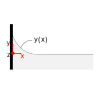
\includegraphics[width=0.85\textwidth, trim=0 80 0 50, clip]{./fig/freeSurfaceShape}
 \end{center}
\end{minipage}

\sol

\noindent
\partone

\noindent
\parttwo

Poiché si studia il problema nelle vicinanze di una parete piana infinita, è lecito assumere che la soluzione non dipenda dalla coordinata che descrive la lunghezza della parete, la coordinata $z$ facendo riferimento al disegno {\color{red} (TODO)}. L'equazione di Young-Laplace per una superficie bidmensionale in uno spazio tridimensionale,
\begin{equation}
 P_1 - P_2 = \gamma \left[ \dfrac{1}{R_1} + \dfrac{1}{R_2} \right] \ ,
\end{equation}
si riduce al caso di una superficie monodimensionale in uno spazio bidimensionale, la superficie di contatto è piatta nella direzione $z$. Se $R:=R_1$ è il raggio della superficie nei piani paralleli al piano $x-y$ e $R_2$ il raggio della superficie nei piani paralleli al piano $z-y$, l'equazione di Young-Laplace si riduce a
\begin{equation}
  P_1 - P_2 = \dfrac{\gamma}{R} =: \gamma \, k  \ ,
\end{equation}
poiché $R_2 \rightarrow \infty$, poiché la quota della superficie di contatto non varia al variare di $z$, mantenendo $x$ fissato, e quindi il raggio di curvatura della superficie in quella direzione è infinito. \'E stata introdotta la definizione della curvatura $k := 1/R$.

La pressione nell'aria è costante e uguale al valore della pressione ambiente $P_2 = P_a$.
Si può calcolare la pressione $P_1(x)$ dell'acqua a contatto con la superficie utilizzando la legge di Stevino,
\begin{equation}
  P_1(x) - P_a = \rho g y(x) \ ,
\end{equation}
essendo $y(x)$ la quota della superficie, rispetto alla quota di riferimento $y=0$, scelta come la quota alla quale la pressione dell'acqua è uguale alla pressione $P_a$. Utilizzando l'espressione di $P_1$ e $P_2$, l'equazione di Laplace-Young diventa
\begin{equation}
 \rho g y(x) = \gamma k(x) \ .
\end{equation}
Ricordando che la curvatura di una superficie rappresentata dalla funzione $y(x)$ può essere espressa come {\color{red} (TODO: aggiungere i dettagli ?)},
\begin{equation}
 k(x) = \dfrac{y''(x)}{\left( 1 + y'(x)^2 \right)^{3/2}} \ ,
\end{equation}
si ricava il problema differenziale che descrive la forma della superficie di contatto,
\begin{equation}
\begin{cases}
 \rho g y(x) - \dfrac{y''(x)}{\left( 1 + y'(x)^2 \right)^{3/2}} = 0 \\
 y'(x=0) = -\dfrac{1}{\tan\theta} \\
 y(x\rightarrow \infty) \rightarrow 0
\end{cases}
\end{equation}
con l'equazione di Young-Laplace accompagnata dalla condizione al contorno a parete, in $x=0$, che lega la derivata della superficie all'angolo di contatto, e dalla condizione all'infinito che identifica la quota del pelo libero lontano dalla parete come la quota alla quale la pressione è uguale alla pressione ambiente.
%
\newline \noindent
Definendo la costante $a^2:=\frac{2\gamma}{\rho g}$ e integrando una volta l'equazione differenziale si ottiene
\begin{equation}
 \dfrac{y^2}{a^2} + \dfrac{1}{(1 + y'(x)^2)^{1/2}} = A \ ,
\end{equation}
dove $A$ rappresenta la costante di integrazione. Affinchè la quota della superficie tenda alla quota di riferimento a grande distanza della parete, $y(x\rightarrow\infty) \rightarrow 0$, ``con una sensata regolarità'', è necessario che anche la sua pendenza si annulli, $y'(x\rightarrow\infty) \rightarrow 0$. Questa condizione impone il valore della costante di integrazione, $A = 1$. Integrando nuovamente l'equazione,
\begin{equation}
 \dfrac{y^2}{a^2} + \dfrac{1}{(1 + y'(x)^2)^{1/2}} = 1 \ ,
\end{equation}
si ottiene la soluzione del problema {\color{red} (TODO: aggiungere i dettagli)},
\begin{equation}
 \dfrac{1}{\sqrt{2 a^2 - y(x)^2}} +
 \dfrac{a}{\sqrt{2}} \, \text{Ch}^{-1} \left( \dfrac{\sqrt{2} a}{y(x)} \right) = x + B \ ,
\end{equation}
con la costante di integrazione $B$ da calcolare utilizzando la condizione al contorno a parete.

\vspace{1.0cm}
\noindent
\textbf{Osservazione.} Questo problema fornisce un esempio di calcolo della forma della superficie di contatto tra due fluidi. Nonostante il problema studiato sia uno dei più semplici che si possano immaginare, la sua soluzione analitica richiede già un notevole impegno. Coloro che nutrono passione per l'argomento, sono invitati a calcolare la forma dell'interfaccia tra acqua e aria in un dominio delimitato da due pareti verticali, risolvendo numericamente (esiste una soluzione analitica anche per questo problema, ma risulta ancora più ``criptica'' di quella ricavata per il problema con una sola parete) il problema differenziale non lineare,
\begin{equation}
\begin{cases}
 \rho g y(x) - \dfrac{y''(x)}{\left( 1 + y'(x)^2 \right)^{3/2}} = 0 \quad , \qquad x \in [0,\,L] \\
 y'(x=0) = -\frac{1}{\tan\theta} \\
 y'(x=L) =  \frac{1}{\tan\theta} \\
\end{cases}
\end{equation}

